%% Copyright 2018 H.\ Rabus
%
% This work may be distributed and/or modified under the
% conditions of the LaTeX Project Public License, either version 1.3
% of this license or (at your option) any later version.
% The latest version of this license is in
%   http://www.latex-project.org/lppl.txt
% and version 1.3 or later is part of all distributions of LaTeX
% version 2005/12/01 or later.
%
% This work has the LPPL maintenance status `author-maintained'.
%
% This work consists of the file texbsp.tex
%

\documentclass[smallheadings]{scrartcl}

%%% GENERAL PACKAGES %%%%%%%%%%%%%%%%%%%%%%%%%%%%%%%%%%%%%%%%%%%%%%%%%%%%%%%%%%
% inputenc allows the usage of non-ascii characters in the LaTeX source code
\usepackage[utf8]{inputenc}
\usepackage{graphicx} 
%\graphicspath{ {/u/hnatiuka/Praktikum/PPI/} }



% title of the document
\title{Bericht zu Serie 1}
% optional subtitle
%\subtitle{Draft from~\today}
% information about the author
\author{%
  Arsen Hnatiuk,\\%
  Max Huneshagen 
}
\date{\today} 


%%% LANGUAGE %%%%%%%%%%%%%%%%%%%%%%%%%%%%%%%%%%%%%%%%%%%%%%%%%%%%%%%%%%%%%%%%%%
% babel provides hyphenation patterns and translations of keywords like 'table
% of contents'
\usepackage[ngerman]{babel}

%%% HYPERLINKS %%%%%%%%%%%%%%%%%%%%%%%%%%%%%%%%%%%%%%%%%%%%%%%%%%%%%%%%%%%%%%%%
% automatic generation of hyperlinks for references and URIs
\usepackage{hyperref}

%%% MATH %%%%%%%%%%%%%%%%%%%%%%%%%%%%%%%%%%%%%%%%%%%%%%%%%%%%%%%%%%%%%%%%%%%%%%
% amsmath provides commands for type-setting mathematical formulas
\usepackage{amsmath}
% amssymb provides additional symbols
\usepackage{amssymb}
% HINT
% Use http://detexify.kirelabs.org/classify.html to find unknown symbols!

%%% COLORS %%%%%%%%%%%%%%%%%%%%%%%%%%%%%%%%%%%%%%%%%%%%%%%%%%%%%%%%%%%%%%%%%%%%
% define own colors and use colored text
\usepackage[pdftex,svgnames,hyperref]{xcolor}

%%% Code Listings %%%%%%%%%%%%%%%%
% provides commands for including code (python, latex, ...)
\usepackage{listings}
\definecolor{keywords}{RGB}{255,0,90}
\definecolor{comments}{RGB}{0,0,113}
\definecolor{red}{RGB}{160,0,0}
\definecolor{green}{RGB}{0,150,0}
\lstset{language=Python, 
        basicstyle=\ttfamily\small, 
        keywordstyle=\color{keywords},
        commentstyle=\color{comments},
        stringstyle=\color{red},
        showstringspaces=false,
        identifierstyle=\color{green},
        }


\usepackage{paralist}
\usepackage{nicefrac}
% setting the font style for input und returns in description items
\newcommand{\initem}[2]{\item[\hspace{0.5em} {\normalfont\ttfamily{#1}} {\normalfont\itshape{(#2)}}]}
\newcommand{\outitem}[1]{\item[\hspace{0.5em} \normalfont\itshape{(#1)}]}
\newcommand{\bfpara}[1]{
	
	\noindent \textbf{#1:}\,}

\begin{document}

% generating the title page
\maketitle
% generating the table of contents (requires to run pdflatex twice!)
\tableofcontents
\bigskip

\hrule
\hrule

%%% BEGIN OF CONTENT %%%%%%%%%%%%%%%%%%%%%%%%%%%%%%%%%%%%%%%%%%%%%%%%%%%%%%%%%%

\section{Einleitung}
Aus der Theorie der Taylorentwicklung kann man ein günstiges Verfahren zur Approximation der ersten und zweiten Ableitungen einer Funktion ableiten: 
\begin{align}
\label{eq:1_abl}
f'(x)=\underbrace{\frac{f(x+h)-f(x)}{h}}_{:=D_h^{(1)}(x)}+\mathcal{O}(h)
\end{align}
bzw.
\begin{align}
\label{eq:2_abl}
f''(x)=\underbrace{\frac{f(x+h)-2f(x)+f(x-h)}{h^2}}_{:=D_h^{(2)}(x)}+\mathcal{O}(h^2)
\end{align}
mit der Differenziationsschrittweite $h$.

Dieses Verfahren kann sehr nützlich in der numerischen Mathematik sein, jedoch hängt seine Genauigkeit, wie bei jedem Approximationsverfahren, stark von dem Wert der eingegebenen Parameter ab. Deswegen wird eine Studie der Genauigkeit für die sinnvolle Nutzung des Verfahrens benötigt. Die im Teil 1 erstellten Skripte (\texttt{differenzieren.py} und \texttt{hauptprogramm.py}) erlauben eine numerische Analyse von der Beziehung zwischen der Genauigkeit und den Parametern. Nun führen wir die Analyse aus.

\section{Theorie}
Wie schon gesagt, lassen sich die Formeln \ref{eq:1_abl} und \ref{eq:2_abl} aus der Theorie der Taylorentwicklung ableiten. Diese lautet, dass für eine glatte reellwertige Funktion $f$, für $x\in\mathbb{R}$ und für $h$ in einer passenden Umgebung von $x$, gilt
\[f(x+h)=\sum_{k=0}^{\infty}\frac{f^{(k)}(x)}{k!}h^k=f(x)+f'(x)h+\sum_{k=2}^{\infty}\frac{f^{(k)}(x)}{k!}h^k\]
Das Lösen nach $f'(x)$ liefert
\[f'(x)=\frac{f(x+h)-f(x)}{h}-\sum_{k=2}^{\infty}\frac{f^{(k)}(x)}{k!}h^{k-1}=\frac{f(x+h)-f(x)}{h}+\mathcal{O}(h)\]
Die zweite Formel bekommt man auf eine ähnliche Weise. Wir können die Taylorentwicklung auf ein negatives $h$ anwenden:
\[f(x-h)=\sum_{k=0}^{\infty}\frac{f^{(k)}(x)}{k!}(-h)^k=f(x)-f'(x)h+\frac{f''(x)h^2}{2} +\sum_{k=3}^{\infty}\frac{f^{(k)}(x)}{k!}(-h)^k\]
Daraus bekommen wir
\[f(x+h)+f(x-h)=2f(x)+f''(x)h^2+\sum_{k=2}^{\infty}\frac{f^{(2k)}(x)}{(2k)!}h^{2k}\]
Und das Lösen nach $f''(x)$ liefert
\[f''(x)=\frac{f(x+h)+f(x-h)-2f(x)}{h^2}+\mathcal{O}(h^2)\]

Ein anderer wichtiger Begriff für die Bearbeitung folgender Experimente ist die Periodizität der Sinus Abbildung und seiner Ableitungen. Zu einem gegebenen $j\in\mathbb{R}$ ist die Periode von $sin(jx)$ gleich $\frac{2\pi}{j}$. Die Ableitungen von $sin(jx)$ verhalten sich auf die gleiche Weise.

\section{Experimente}

\paragraph {Experiment 1}
Für die Veranschaulichung der Genauigkeit der Approximation von den Ableitungen bei Schrittweiten $\frac{\pi}{3}$, $\frac{\pi}{4}$, $\frac{\pi}{5}$ und $\frac{\pi}{10}$ haben wir ein Programm geschrieben, und zwar \texttt{hauptprogramm2.py}, und dieses liefert die Abbildung \ref{Abbildung 1}.

\begin{figure}
	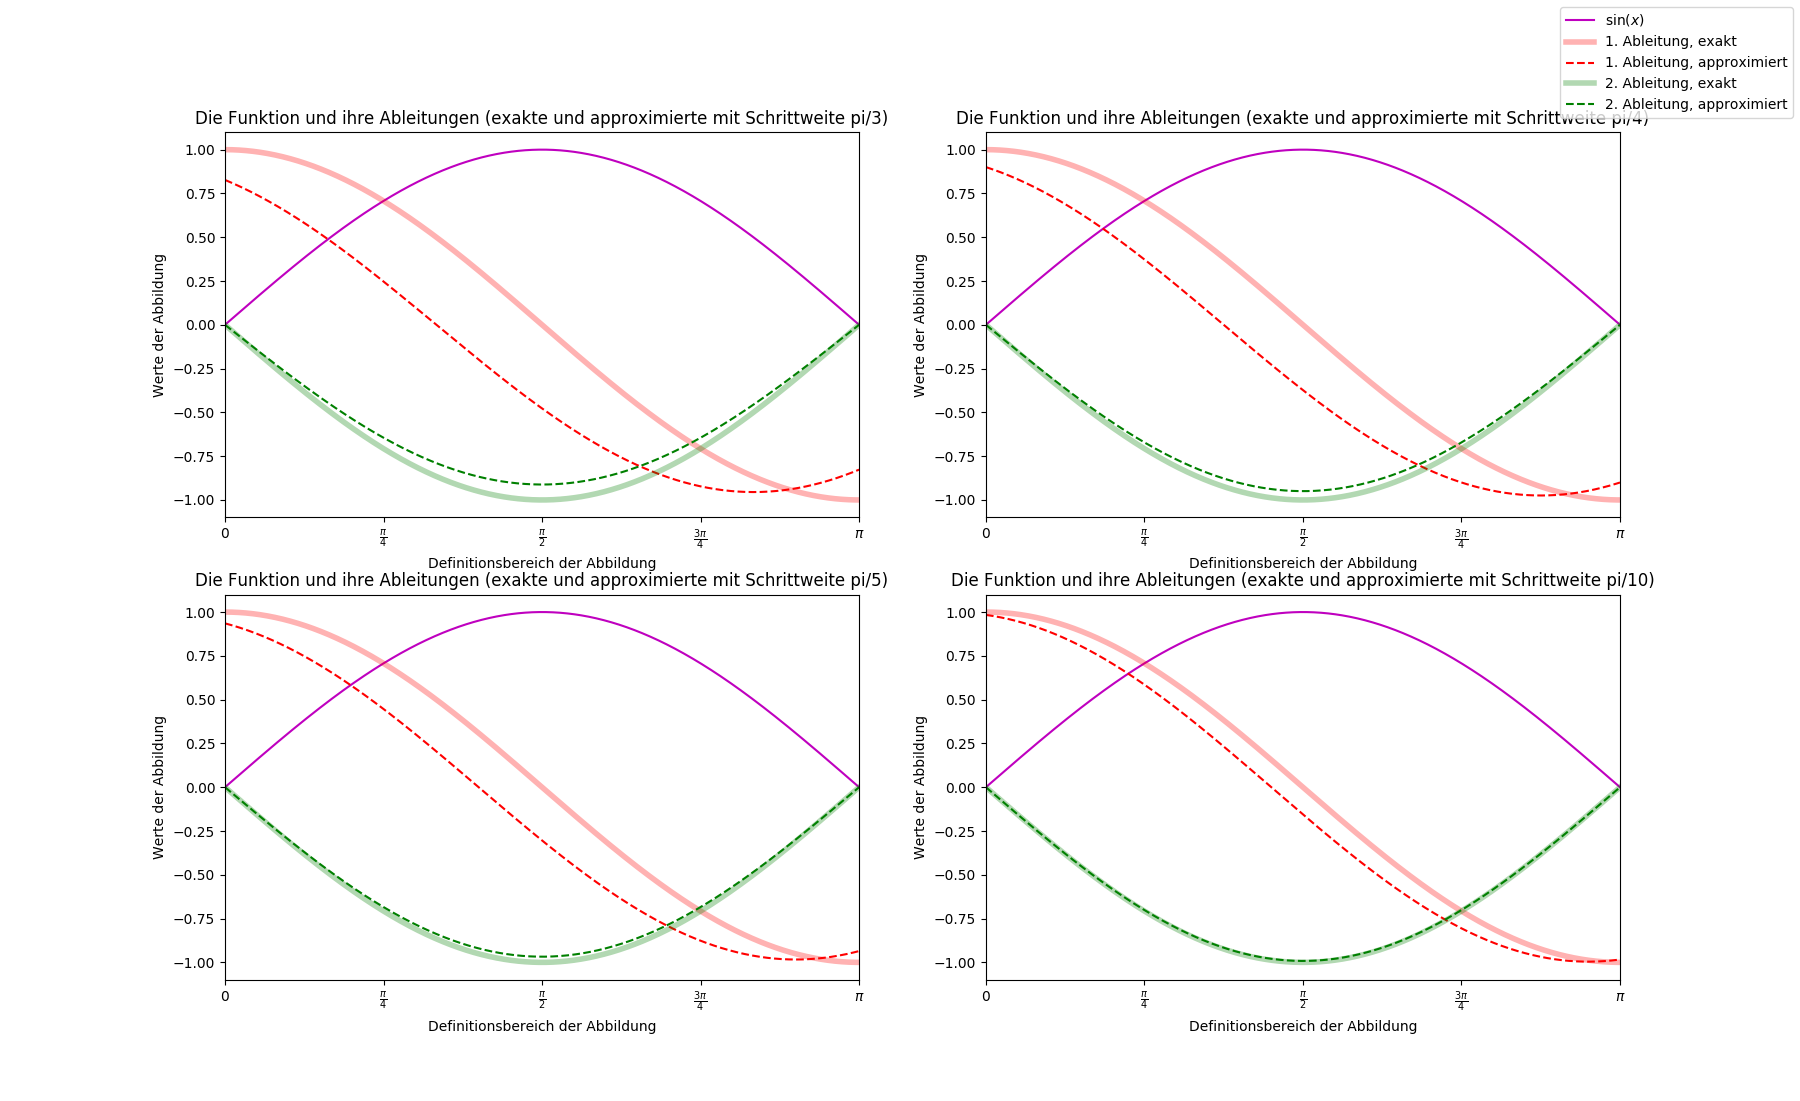
\includegraphics[width=\linewidth]{4Bilder.png}
	\caption{Die approximierten Ableitungen für verschiedene Schrittweiten (Experiment 1).}
	\label{Abbildung 1}
\end{figure}

\section{Analyse der Experimente}

\paragraph{Experiment 1}
Aus der graphischen Ausgabe des ersten Experiments \ref{Abbildung 1} werden drei Sachen ersichtlich. Erstens, die Approximation der beiden Ableitungen wird genauer, je kleiner die Schrittweite. Dies stimmt mit der Theorie überein, weil wir erwarten, dass der Fehler in der ersten bzw. zweiten Ableitung der Ordnung $\mathcal{O}(h)$ bzw. $\mathcal{O}(h^2)$ ist, insbesondere proportional zur Schrittweite $h$ für kleine $h$. \newline
Zweitens, die Approximation der ersten Ableitung ist im Vergleich zu den genauen Daten nach Rechts verschoben. Dies ist auch erwartet und der Grund dafür liegt in der Approximationsformel für die erste Ableitung \ref{eq:1_abl}. Und zwar sieht man, dass die approximierte Tangente nicht um den Punkt $x$ zentriert ist, sondern um den Mittelpunkt zwischen $x+h$ und $x$. Folglich ist die Approximation um $\frac{h}{2}$ nach rechts verschoben. Dies passiert nicht bei der zweiten Ableitung, weil die entsprechende Formel \ref{eq:2_abl} sowohl auf $x+h$, als auch auf $x-h$ beruht. \newline
Schließlich ist die Approximation der zweiten Ableitung für diese Schrittweiten genauer, als die erste. Wie die erste Beobachtung, liegt dies auf die Ordnung der entsprechenden Fehler. Für $h=\frac{\pi}{4}$, $\frac{\pi}{5}$ und $\frac{\pi}{10}$ ist $h^2<h$, und folglich soll die Approximation der zweiten Ableitung genauer sein, als die erste. Für $h=\frac{\pi}{3}$ lässt sie die höhere Genauigkeit der zweiten Ableitung durch die oben beschriebene Verschiebung in der ersten Ableitung erklären. 

\paragraph{Experiment 2}
%hier Referenz zu Abbildung 2 zu schreiben
Der Fehlerplot zeigt drei verschiedene Tendenzen im Fehlerverhalten in Abhängigkeit von der Schrittweite. In dem mittleren Bereich der Schrittweite (ungefähr für $h\in\left[10^{-8}, 1\right]$ für die erste Ableitung und $h\in[10^{-3}, 1] $ für die zweite) verhält sich der Fehler genau so, wie es die Approximationsformeln andeuten - er ist proportional zu der Schrittweite, und zwar linear im Fall der Approximation der ersten Ableitung und quadratisch im Fall der Approximation der zweiten Ableitung. \newline
Dieses Verhalten ändert sich bei Schrittweiten, die größer als 1 sind. In diesem Bereich konvergiert der Fehler für beide Approximationen allmählich gegen 1. Der Grund dafür lässt sich auch aus den Formeln ablesen. Da wir mit der Sinus Funktion arbeiten, kann $f(x+h)-f(x)$ betragsmäßig niemals größer als 2 sein. Analog ist der Betrag von $f(x+h)-2f(x)+f(x-h)$ durch 4 beschränkt. Folglich geht bei wachsendem $h$ der Approximierte Wert der beiden Ableitungen für alle Punkte $x$ gegen 0. Da diese Werte mit denen der Kosinus bzw. negativen Sinus Abbildungen verglichen werden (diese bleiben immer im Intervall $[-1, 1]$), konvergiert der maximale Fehler gegen 1. \newline
Ein ganz anderes Verhalten des Fehlers beobachtet man für sehr kleine Schrittweiten (kleiner als $10^{-8} $ für die erste und $10^{-3}$ für die zweite Abbildungen). Der erste Grund dafür ist dass die Sinus Abbildung in kleinen Umgebungen um ihre Extrema sehr flach ist. Der zweite Grund ist dass die \texttt{numpy.sin} Funktion, die wir in unserer Implementierung benutzen, während arithmetischer Operationen nur 16 Stellen Genauigkeit benutzt (das haben wir durchs Rechnen herausgefunden: \texttt{numpy.sin(1)-numpy.sin(1+10**-17)}  liefert \texttt{0}). Folglich unterscheiden sich \texttt{sin(x+h)} und \texttt{sin(x)} für kleinen $h$ in einer Umgebung von $\frac{\pi}{2}$ nur um die allerletzten Nachkommastellen. Also hat der Ausdruck \texttt{sin(x+h)-sin(x)} für genügend kleine Werte von $h$ nur eine oder zwei Stellen Genauigkeit. Das gleiche gilt auch für \texttt{sin(x-h)+sin(x+h)-2*sin(h)}. Wenn diese approximierte Werte dann mit den exakten verglichen werden, kommt ein immer größer Fehler raus (und zwar ein sehr großer Fehler bei der Approximation der zweiten Ableitung, weil diese Werte nicht um $h^{-1}$, sondern um $h^{-2}$ skaliert wird). Man sieht eine andere Auswirkung der Arithmetik mit 16-stelliger Genauigkeit bei dem Verhalten des Fehlers für $h=10^{-16}$. Für beide Ableitungen ist der Fehler in diesem Fall 1. Dies liegt daran, dass \texttt{sin(x)=sin(x + 10**-16)}, also die approximierten Werten sind immer 0. Wie im Fall der großen $h$, ist der Fehler dann immer 1.

\section{Zusammenfassung}

%%% END OF DOCUMENT %%%%%%%%%%%%%%%%%%%%%%%%%%%%%%%%%%%%%%%%%%%%%%%%%%%%%%%%%%%
\end{document}
